\section{Future work} \label{sec:futurework}

The goal of this work is to reliably reproduce nuclear shape deformations. This requires a symmetry break in the system governing laminar assembly/disassembly dynamics. We plan to achieve this by including a feedback term in the functions $k_{off}^{a,b}$. Hypothesized sources of feedback include competition between lamin types, and stress induced feedback. These ideas are shown schematically in Fig. ~\ref{fig::feedback}. Once we have established a symmetry break, we will explore perturbations to the model which correspond to physical changes  in the lamin A/C protein which can best reproduce patient versus control data. These potential perturbations are summarized in Table ~\ref{tab:perturbations}


\begin{figure}[h]
\centering
\captionsetup{width=.9\linewidth}
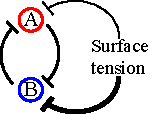
\includegraphics[width=4in]{Project3/figs/feedback_stretch.pdf}
\caption{feedback.}
\label{fig::feedback}
\end{figure}


\begin{table}[t!]
\caption{Potential perturbations.}\centering \label{tab:perturbations} 
\begin{tabular}{ l  l}
\hline
Model perturbation & Change in lamin A/C \\
\hline
Decrease total amount of lamin A/C  & Haploinsufficiency  \\
Modify assembly/disassembly rates & Structural change leading to abnormal localization of lamin\\
Modify $\mathcal{G}_a$ (elastic modulus) & Weaken molecular strength of Lamin A/C  \\
Modify $\mathcal{M}_a$ (bending modulus)& Weaken Lamin A/C-Lamin A/C crosslinking  \\
Modify $\mathcal{F}_{cyto}, \sigma_{\rm VM}$ & Weaken transmembrane link  \\
Modify feedback from lamin B &Modify interaction with Lamin B \\
\hline
\end{tabular}
\end{table}